%% Middle column of the poster, written by scripts/poster_tables.py (do not edit the numbers by hand).
%% Needs tree_figure_pre_date_poster.png in the Overleaf project.
\begin{column}{\colwidth}

\begin{myblock}{Technical Implementation}
\begin{enumerate}
  \item \textbf{Pre-date and in-date feature sets.} \emph{Pre-date:} sign-up answers plus six pair features
  (age gap, interest similarity, same field, same goal, preference fit each way). \emph{In-date:} adds the
  16 ratings the two gave each other.
  \item \textbf{Nested event-level cross-validation.} Missing-value fills, scaling and tuning use only the
  training events.
  \item \textbf{Event-clustered standard errors.} Pairs at one event share people, so each of the 21 events
  is one cluster.
\end{enumerate}
\end{myblock}

\begin{myblock}{Performance by Model}
Held-out AUC (standard error); 0.5 = chance.
\begin{center}\small
\begin{tabular}{lcc}
\toprule
Model & Before the date & With in-date ratings \\
\midrule
Logistic (with splines) & 0.542 (0.020) & 0.780 (0.014) \\
Stepwise logistic & 0.559 (0.023) & 0.835 (0.008) \\
LDA & 0.553 (0.020) & 0.790 (0.012) \\
QDA (regularized) & 0.579 (0.023) & 0.836 (0.008) \\
Lasso & 0.573 (0.018) & 0.838 (0.008) \\
Single tree (depth 3) & 0.533 (0.017) & 0.796 (0.011) \\
\textbf{Random forest} & \textbf{0.583} (0.020) & \textbf{0.846} (0.009) \\
\bottomrule
\end{tabular}
\end{center}
\begin{itemize}
  \item Before the date every model is near chance (AUC 0.53--0.58).
  \item The four-minute date adds about 0.26 to the AUC.
  \item The forest leads, but its lead over the runner-up is within the error bars.
\end{itemize}
\end{myblock}

\begin{myblock}{What the Best Model Uses}
\begin{figure}
\centering
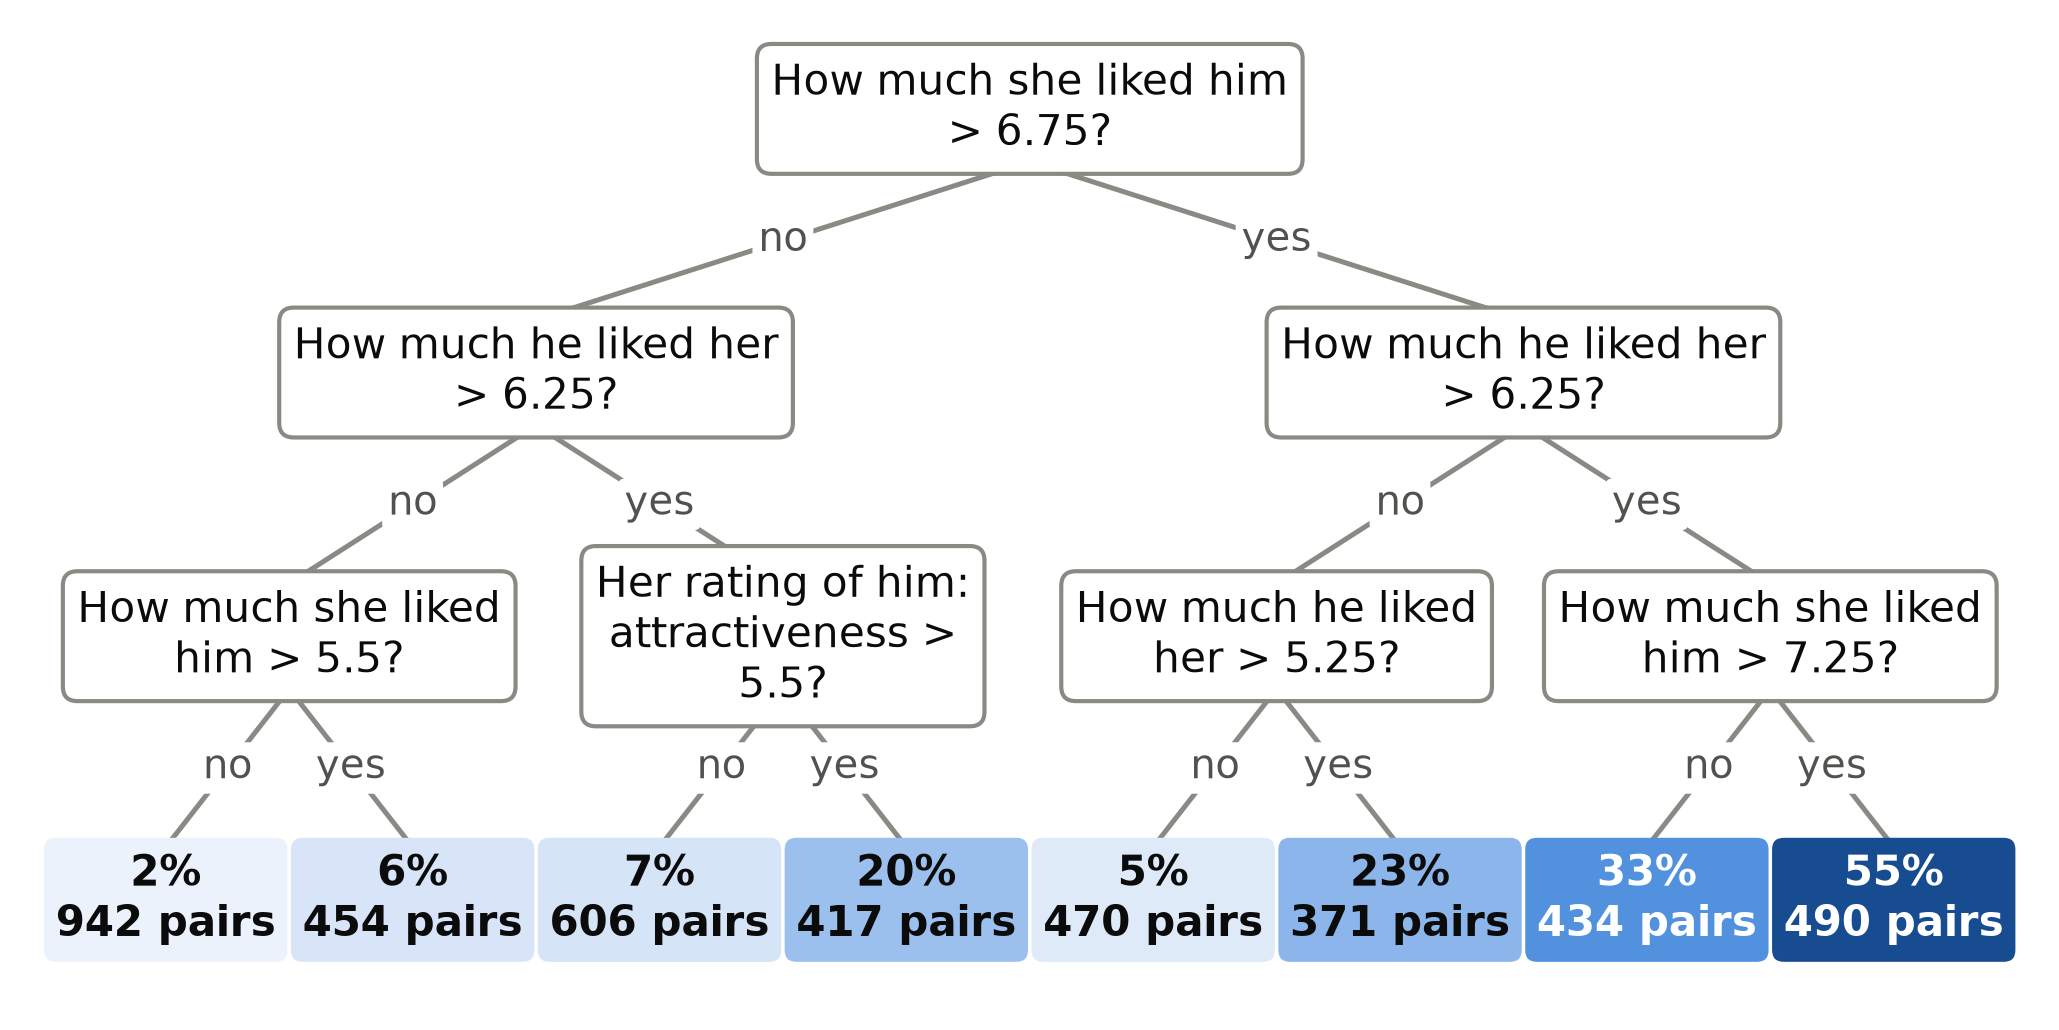
\includegraphics[width=0.92\linewidth]{tree_figure_pre_date_poster.png}
\caption{One 3-level tree fitted to all pairs; leaves give the share that matched. Held out it scores AUC
0.796; the 500-tree forest scores 0.846.}
\end{figure}
\vspace{-0.3cm}
Predictors ranked by how far the forest's held-out AUC falls when each is shuffled:
\begin{center}\small
\begin{tabular}{lc}
\toprule
Predictor & AUC drop (SE) \\
\midrule
\multicolumn{2}{l}{\textit{With in-date ratings (forest AUC 0.846)}} \\
How much he liked her & 0.020 (0.004) \\
How much she liked him & 0.019 (0.005) \\
Her rating of him: fun & 0.013 (0.003) \\
His rating of her: attractiveness & 0.012 (0.002) \\
Her rating of him: attractiveness & 0.011 (0.003) \\
\midrule
\multicolumn{2}{l}{\textit{Before the date (forest AUC 0.583)}} \\
Her stated weight on fun & 0.018 (0.007) \\
How often he dates & 0.014 (0.006) \\
Age gap & 0.006 (0.004) \\
\bottomrule
\end{tabular}
\end{center}
\vspace{-0.2cm}
Liking matters most, then fun and attractiveness. Shuffling all in-date ratings at once drops the AUC by
0.34; all sign-up answers, by 0.008.
\end{myblock}

\end{column}
